\section{HRS Calibration}
 After exiting the target chamber, a charged particle travels a long distance within the magnets of the HRS, and its trajectory after the Q3 exit is determined by two VDCs placed at the focal plane of the HRS. By using the focal plane quantities, an optics matrix reconstructs the particle's position and direction in the target plane where the electron interacts with the target.

 The standard HRS optics matrices have already been optimized in previous Hall-A experiments. However, the absolute positions of the target, the HRS and detectors change from time to time, so these offsets should be taken into account in the optics matrices. Furthermore, during the E08-014, the momentum of the third quadrupole in HRS-R (RQ3) was limited to 2.8273 GeV/c due to a power supply issue, while our maximum momentum setting was 3.055 GeV/c. The RQ3 field had to be scaled down to 87.72\% of the dipole field for each setting. Therefore, the previous HRS-R optics matrix was not applicable. 
 
 In this section, a calibration procedure to obtain new optics matrices for this experiment will be introduced.

\subsection{Coordinate Systems}
  \begin{figure}[!ht]
    \begin{center}
      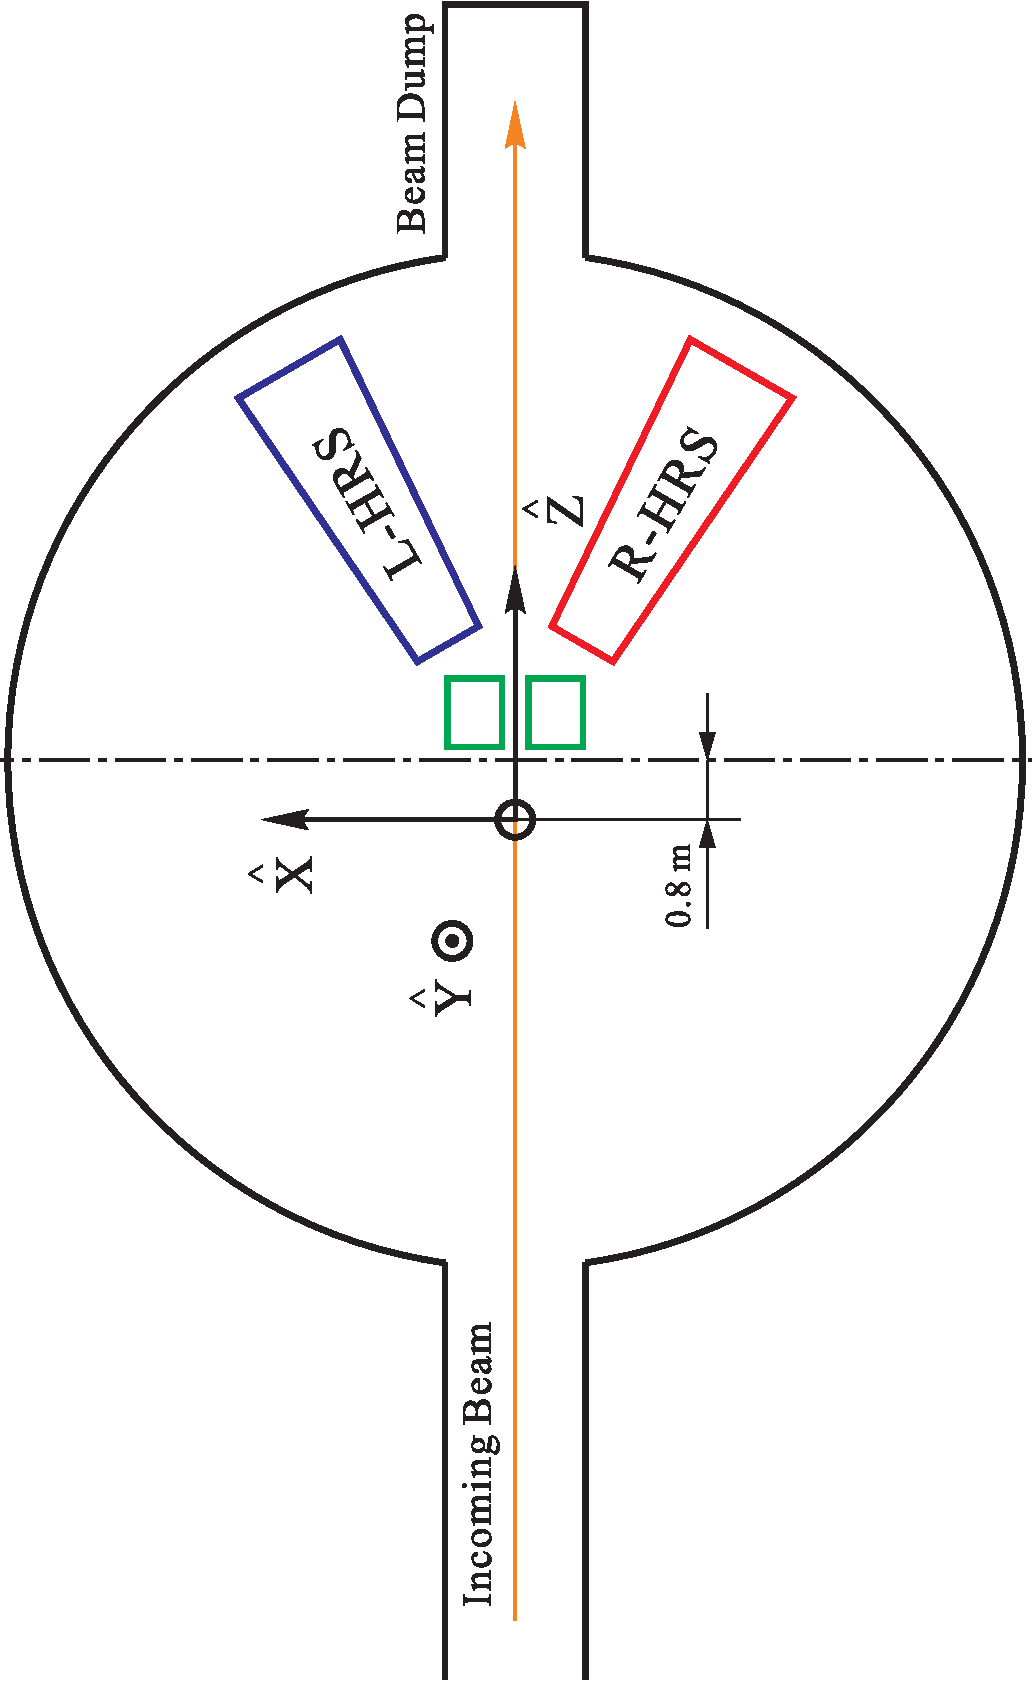
\includegraphics[type=pdf,ext=.pdf,read=.pdf,angle=270,width=0.60\textwidth]{./figures/optics/HCS_new}
      \caption[Hall coordinate system (HCS)]{\footnotesize{Hall coordinate system (HCS), which defines the beam position and the target location with respect to the hall center which is given as the intersection of the beam and the vertical axis of the target system. $\hat{x}$ is to the left of the beam direction, $\hat{z}$, and $\hat{y}$ is vertically up.}}
      \label{HCS}
    \end{center}
  \end{figure}
 The coordinates used during data analysis are briefly presented here. A more detailed description of Hall A coordinate systems and the translation between coordinates is given in Ref.~\cite{nilanga_optics}. Notes that angles defined in all coordinates are the tangent of their values.
\begin{itemize}
\item \textbf{Hall Coordinate System (HCS)} \\
  The center of the HCS is defined as the intersection of the beam and the vertical axis of the target system. $\hat{z}$ is along the direction of the beam, $\hat{x}$ is to the left of $\hat{z}$ and $\hat{y}$ is vertically up (Fig.\ref{HCS}).
  \begin{figure}[!ht]
    \begin{center}
      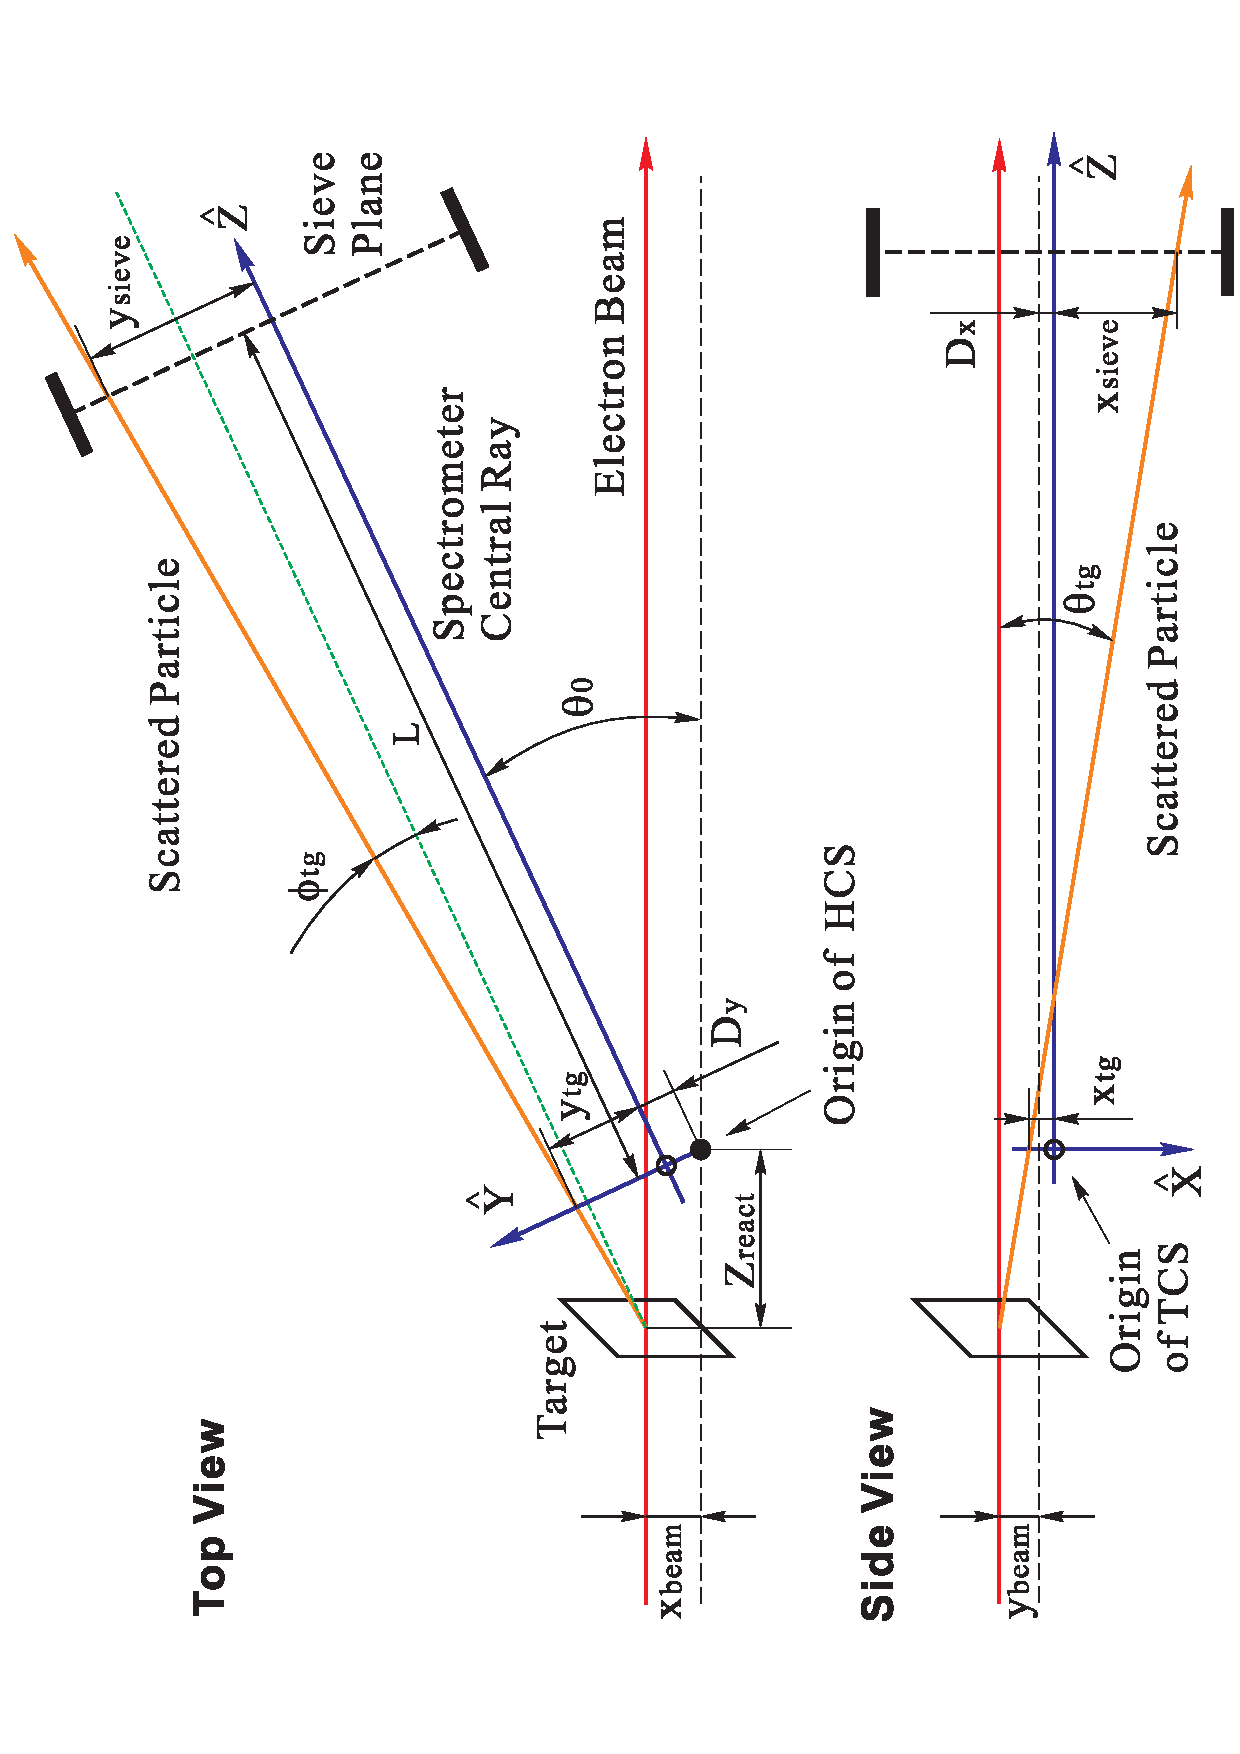
\includegraphics[type=pdf,ext=.pdf,read=.pdf,angle=270,width=0.85\textwidth]{./figures/optics/TCS}
      \caption[Target coordinate system (TCS)]{\footnotesize{Target coordinate system (TCS). $\hat{z}$ goes from the target system perpendicularly to the center hole of the sieve slit plane attached to the Q1 entrance of each HRS. The intersection of $\hat{z}$ and the vertical axis of the target system defines the origin, hence there is a potential offset between the hall center and the origin of TCS. $\hat{x}$ is normal to $\hat{z}$ and points down, and $\hat{y}$ is to the left of $\hat{z}$.}}
      \label{TCS}
    \end{center}
  \end{figure}
    \begin{figure}[!ht]
    \begin{center}
      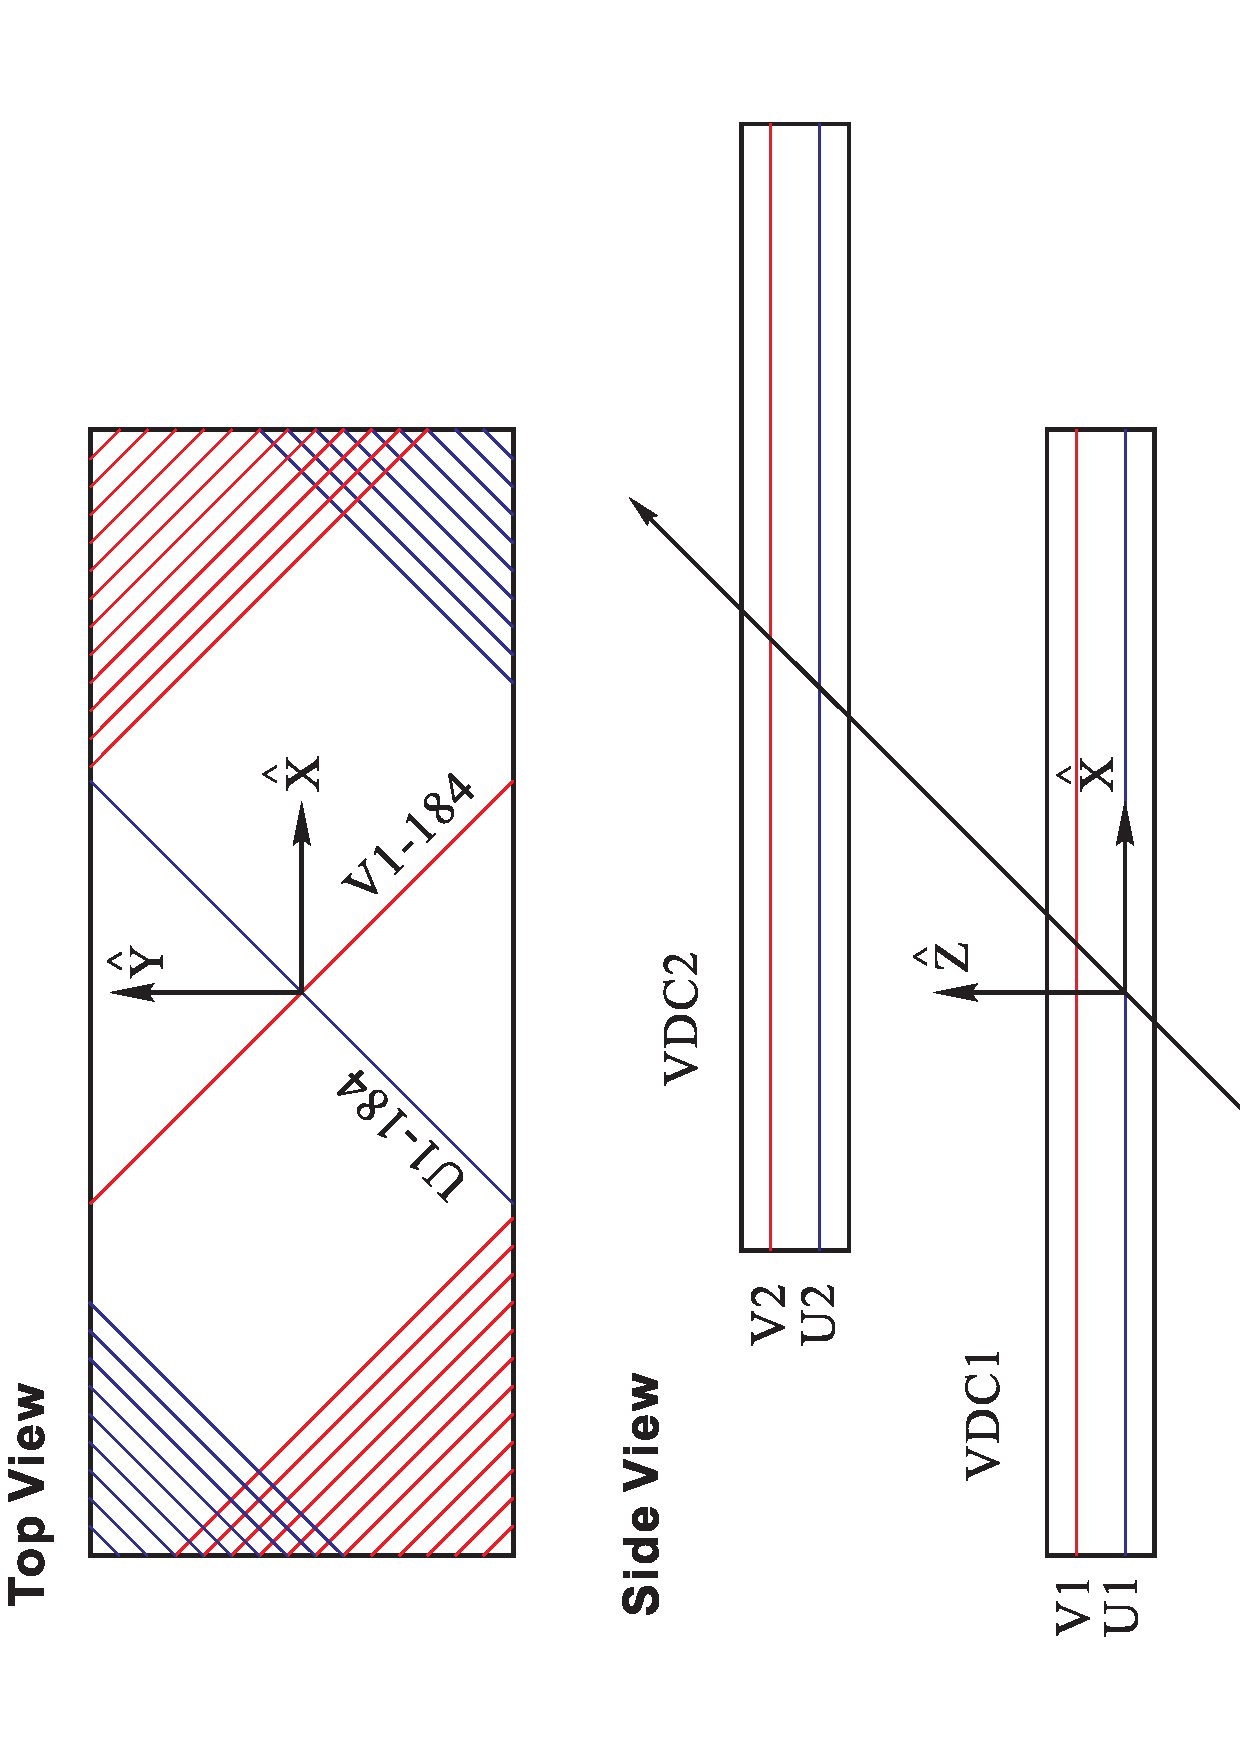
\includegraphics[type=pdf,ext=.pdf,read=.pdf,angle=270,width=0.7\textwidth]{./figures/optics/DCS}
      \caption[Detector coordinate system (DCS)]{\footnotesize{Detector coordinate system (DCS). Its origin is given by the intersection of wire-184 of U1 and wire 184 of V1. $\hat{z}$ is perpendicular to the VDCs, $\hat{x}$ is horizontally along the long edge of the VDC and points away from the hall center, and $\hat{y}$} is along the short edge of the VDC and vertically up.}
      \label{DCS}
    \end{center}
  \end{figure}
\item \textbf{Target Coordinate System (TCS)}   \\
  As shown in Fig.\ref{TCS}, $\hat{z_{tg}}$ is the direction from the target system perpendicular through the center hole in the sieve slit plane on each spectrometer. The origin of TCS is given by the intersection of $\hat{z}_{tg}$ and the vertical axis of the target system, and $L$ is a constant length from the origin of TCS to the sieve slit plane. $\hat{x}_{tg}$ is parallel to the sieve slit plane and vertically down, and $\hat{y}_{tg}$ is to the left of $\hat{z}_{tg}$. $\hat{\theta}_{tg}$ (the out-of-plane angle) and $\hat{\phi}_{tg}$ (the in-plane angle) are taken to be $dx_{sieve}/L$ and $dy_{sieve}/L$. The origins of HCS and TCS are not necessarily in the same location and the value of \emph{D},  the offset between two positions, changes when moving HRSs to different angles. Surveys are required during the experiment running to obtain the offset value.
    \begin{figure}[!ht]
    \begin{center}
      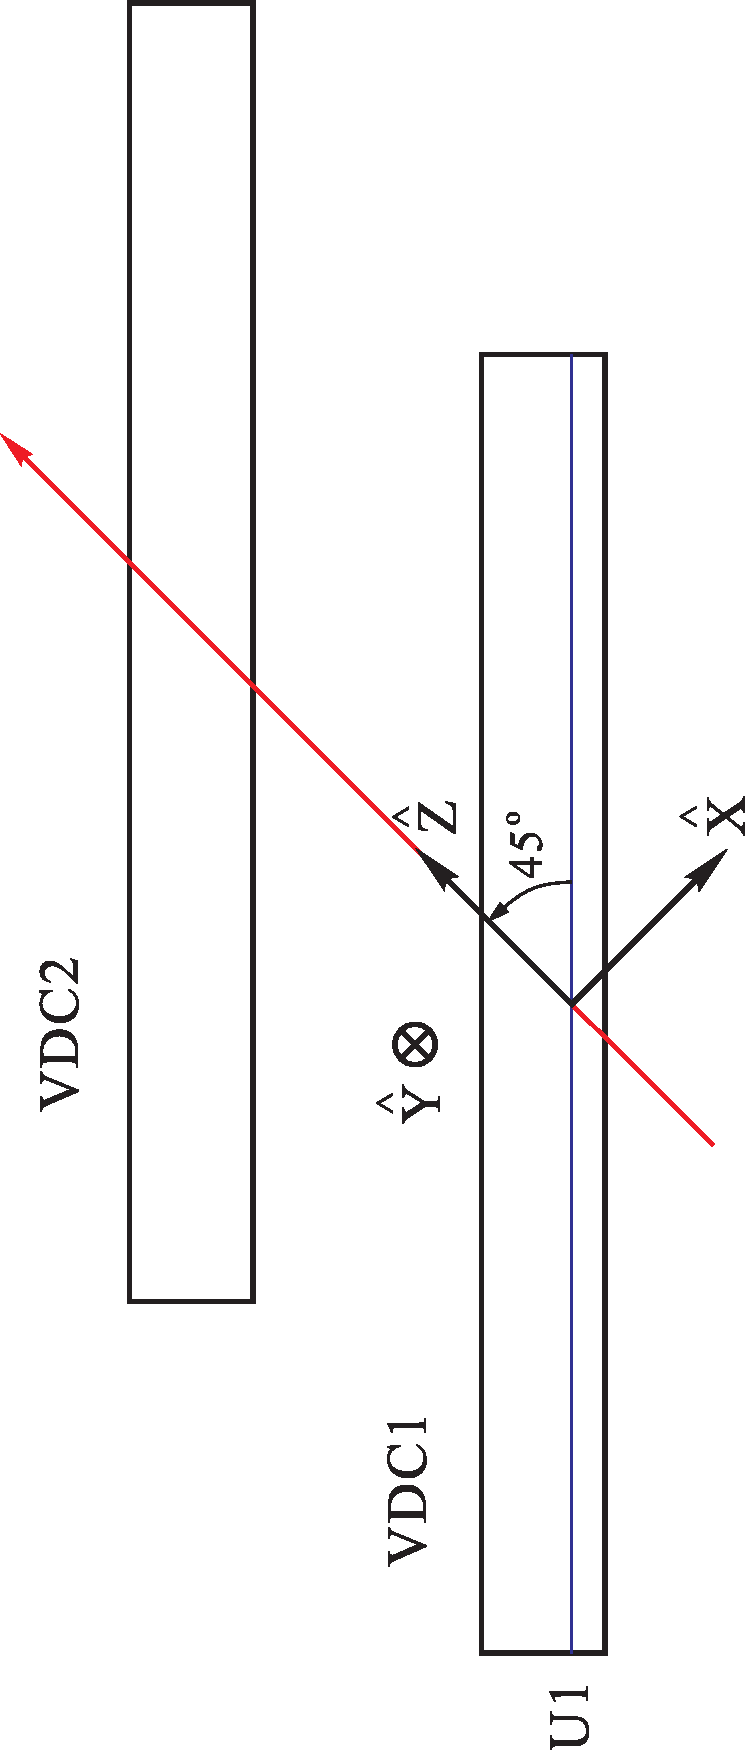
\includegraphics[type=pdf,ext=.pdf,read=.pdf,angle=270,width=0.60\textwidth]{./figures/optics/TRCS_new}
      \caption[Transport coordinate system (TRCS)]{\footnotesize{Transport coordinate system (TRCS), which is generated by rotating the DCS clockwise around  $\hat{y_{det}}$ by $45^{\circ}$.}}
      \label{TRCS}
    \end{center}
  \end{figure}
    \begin{figure}[!ht]
    \begin{center}
      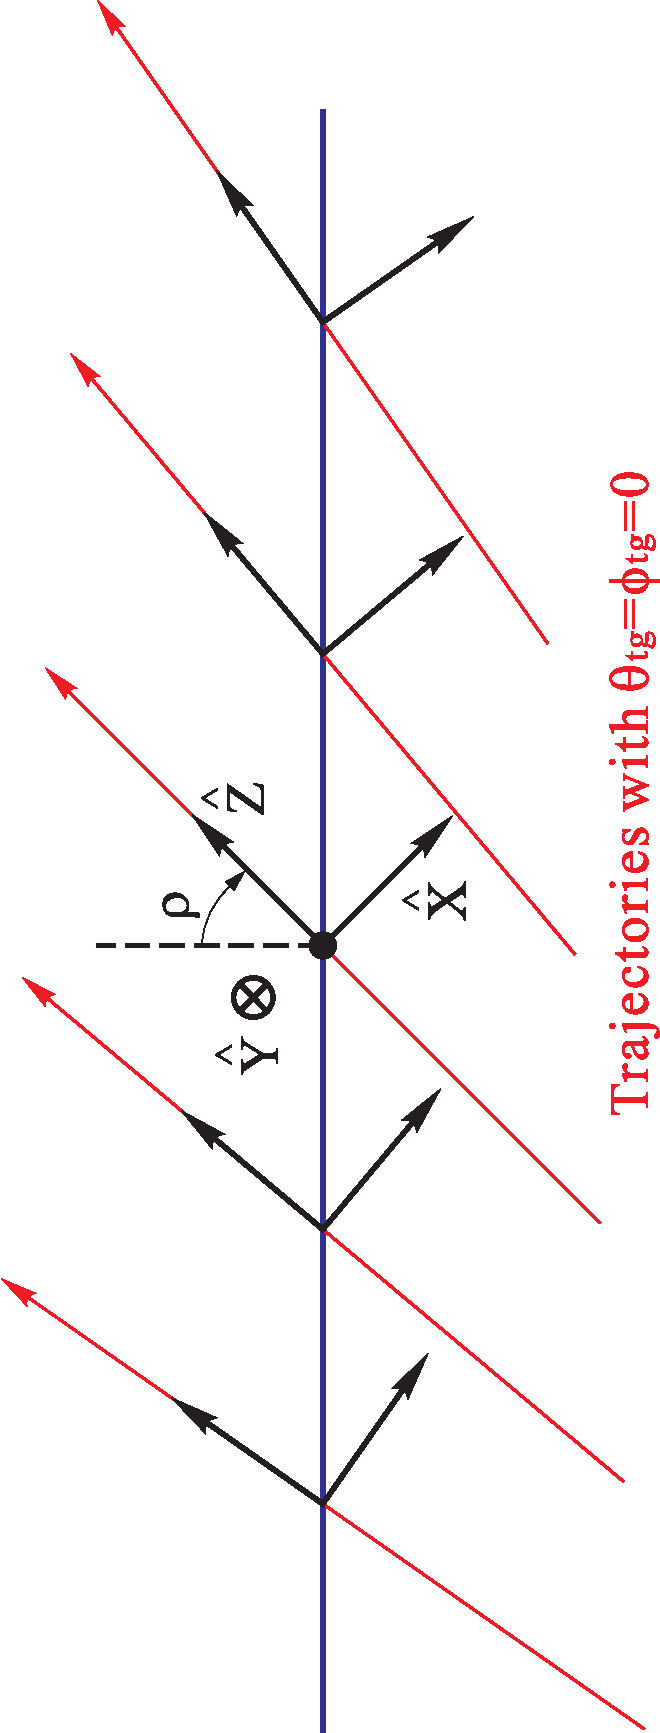
\includegraphics[type=pdf,ext=.pdf,read=.pdf,angle=270,width=0.65\textwidth]{./figures/optics/FCS_new}
      \caption[Focal plane coordinate system (FCS)]{\footnotesize{Focal plane coordinate system (FCS), obtained from rotating DCS around its $\hat{y}$ by an angle $\rho$ so $\hat{z}$ is parallel to the central ray with $\hat{\theta}_{tg}$=$\hat{\phi}_{tg}$=0 and $\delta p=(p-p_{0})/p_{0}$.}}
      \label{FCS}
    \end{center}
  \end{figure}
\item \textbf{ Detector Coordinate System (DCS)} \\
  The origin of DCS can be defined as the intersection point of the wire 184 of U1 plane and the wire 184 of V1 plane on the first VDC (VDC1). $\hat{z}_{det}$ is perpendicular to the VDC planes away from HRS, $\hat{x}_{det}$ is horizontally along the long symmetry axis of VDC1 pointing away from the hall center, and $\hat{y}_{det}$ is vertically up toward $\hat{z}_{det}$ (Fig.~\ref{DCS}).

\item \textbf{Transport Coordinate System (TRCS)} \\ 
  The TRCS is generated by rotating the DCS clockwise around  $\hat{y_{det}}$ by $45^{\circ}$ (Fig.~\ref{TRCS}).

\item \textbf{Focal Plane Coordinate System (FCS)} \\
  The FCS is obtained by rotating DCS around its $\hat{y}_{det}$ axis by an angle $\rho$, which is the angle between $\hat{z}_{det}$ axis and the local central ray with $\hat{\theta}_{tg}$=$\hat{\phi}_{tg}$=0 for the corresponding relative  momentum $\delta p=(p-p_{0})/p_{0}$ (Fig.\ref{FCS}).

\end{itemize}

\subsection{Optics Optimization}
The optics calibration follows the procedure described in Ref.~\cite{nilanga_optics}. An optics matrix for HRS is a set of polynomial functions to calculate the target plane quantities, $\delta p$, $y_{tg}$, $\theta_{tg}$ and $\phi_{tg}$, by using the focal plane quantities, $x_{fp}$, $y_{fp}$, $\theta_{fp}$ and $\phi_{fp}$. The functions are given as: 
\begin{eqnarray}
  & &\delta p    = \sum_{i,j,k,l} C^{D}_{ijkl}x^{i}_{fp} \theta^{j}_{fp}y^{k}_{fp}\phi^{l}_{fp}, \\
  & &y_{tg}      = \sum_{i,j,k,l} C^{Y}_{ijkl}x^{i}_{fp} \theta^{j}_{fp}y^{k}_{fp}\phi^{l}_{fp}, \\
  & &\theta_{tg} = \sum_{i,j,k,l} C^{T}_{ijkl}x^{i}_{fp} \theta^{j}_{fp}y^{k}_{fp}\phi^{l}_{fp}, \\
  & &\phi_{tg}   = \sum_{i,j,k,l} C^{P}_{ijkl}x^{i}_{fp} \theta^{j}_{fp}y^{k}_{fp}\phi^{l}_{fp},
  \label{optics_eq}
\end{eqnarray}
where D-terms ($C^{D}_{jkl}$), Y-terms ($C^{Y}_{jkl}$), T-terms ($C^{T}_{jkl}$), and P-terms ($C^{P}_{jkl}$) represent the matrix elements of $\delta p$, $y_{tg}$, $\theta_{tg}$ and $\phi_{tg}$, respectively. An optics calibration procedure is set to determine the matrix elements by using the optics data taken during the experiment.

There are three new variables in HCS which are more practical for long targets and foil targets with known offsets from the hall center:
\begin{eqnarray}
  & & z_{react} = \frac{-\left(y_{tg} + D_{y}\right)+x_{beam}\left(cos\left(\Theta_{0}\right)-\phi_{tg} sin\left(\Theta_{0}\right)\right)}{cos(\Theta_{0})\phi_{tg}+sin(\Theta_{0})}, \\
  & & x_{sieve} = x_{tg} + L\cdot \theta_{tg},\\
  & & y_{sieve} = y_{tg} + L\cdot \phi_{tg},
\end{eqnarray}
where $x_{beam}$ is the horizontal position of the beam, $\theta_{0}$ is the central angle of the spectrometer, and \emph{L} and \emph{D} are defined in TCS. $z_{react}$ is the reaction location along the beam direction and also provides the target position in HCS. $x_{sieve}$ and $y_{sieve}$ represent the vertical and horizontal positions at the sieve slit plane. Table~\ref{optics_offset_table} and Table~\ref{sieve_offset_table} give the values of \emph{D}, $x_{sieve}$ and $y_{sieve}$ from survey reports. During the experiment, the beam position was locked at (-2.668 mm, 3.022 mm).

\begin{table}
  \centering 
  \begin{tabular}{|c||c|c|c|c|c|c|}
    \hline
    &   Angle   &    $D_{x} (mm)$ & $D_{y}$ (mm) & $D_{z} (mm)$ & Survey Report \\
    \hline \hline
    HRS-L & 21.480   & 1.78 & 1.25 & -0.70  & DVCS~\cite{survey_dvcs_2010}\\
    \hline 
    HRS-R & -20.022 & -2.91 & 0.73 & -1.06 & PVDIS~\cite{survey_pvdis_2009}\\
    \hline 
  \end{tabular}
  \caption[Spectrometer offsets from survey reports]{\footnotesize{ Spectrometer offsets for survey reports, where \emph{D}, the offset between the origins of HCS and TCS, is given in term of three components in HCS.}}
  \label{optics_offset_table}
\end{table}

\begin{table}
  \centering
  \begin{tabular}{|c||c|c|c|c|c|c|}
    \hline
    &   L  (mm) &    $x_{sieve} (mm)$ &  $y_{sieve} (mm)$  &  Survey Report\\
    \hline \hline
    HRS-L & 1182.3  & -1.05 & 0.20  & DVCS~\cite{survey_dvcs_2010}\\
    \hline 
    HRS-R & 1175.9  & 1.04  & 0.05 & A1n~\cite{survey_a1n_2009} \\
    \hline 
  \end{tabular}
  \caption[Sieve slit plates offsets from survey reports.]{\footnotesize{ Sieve slit plates offsets from survey reports. The values were measured in HCS.}}
  \label{sieve_offset_table}
\end{table}

\begin{figure}[!ht]
  \begin{center}
    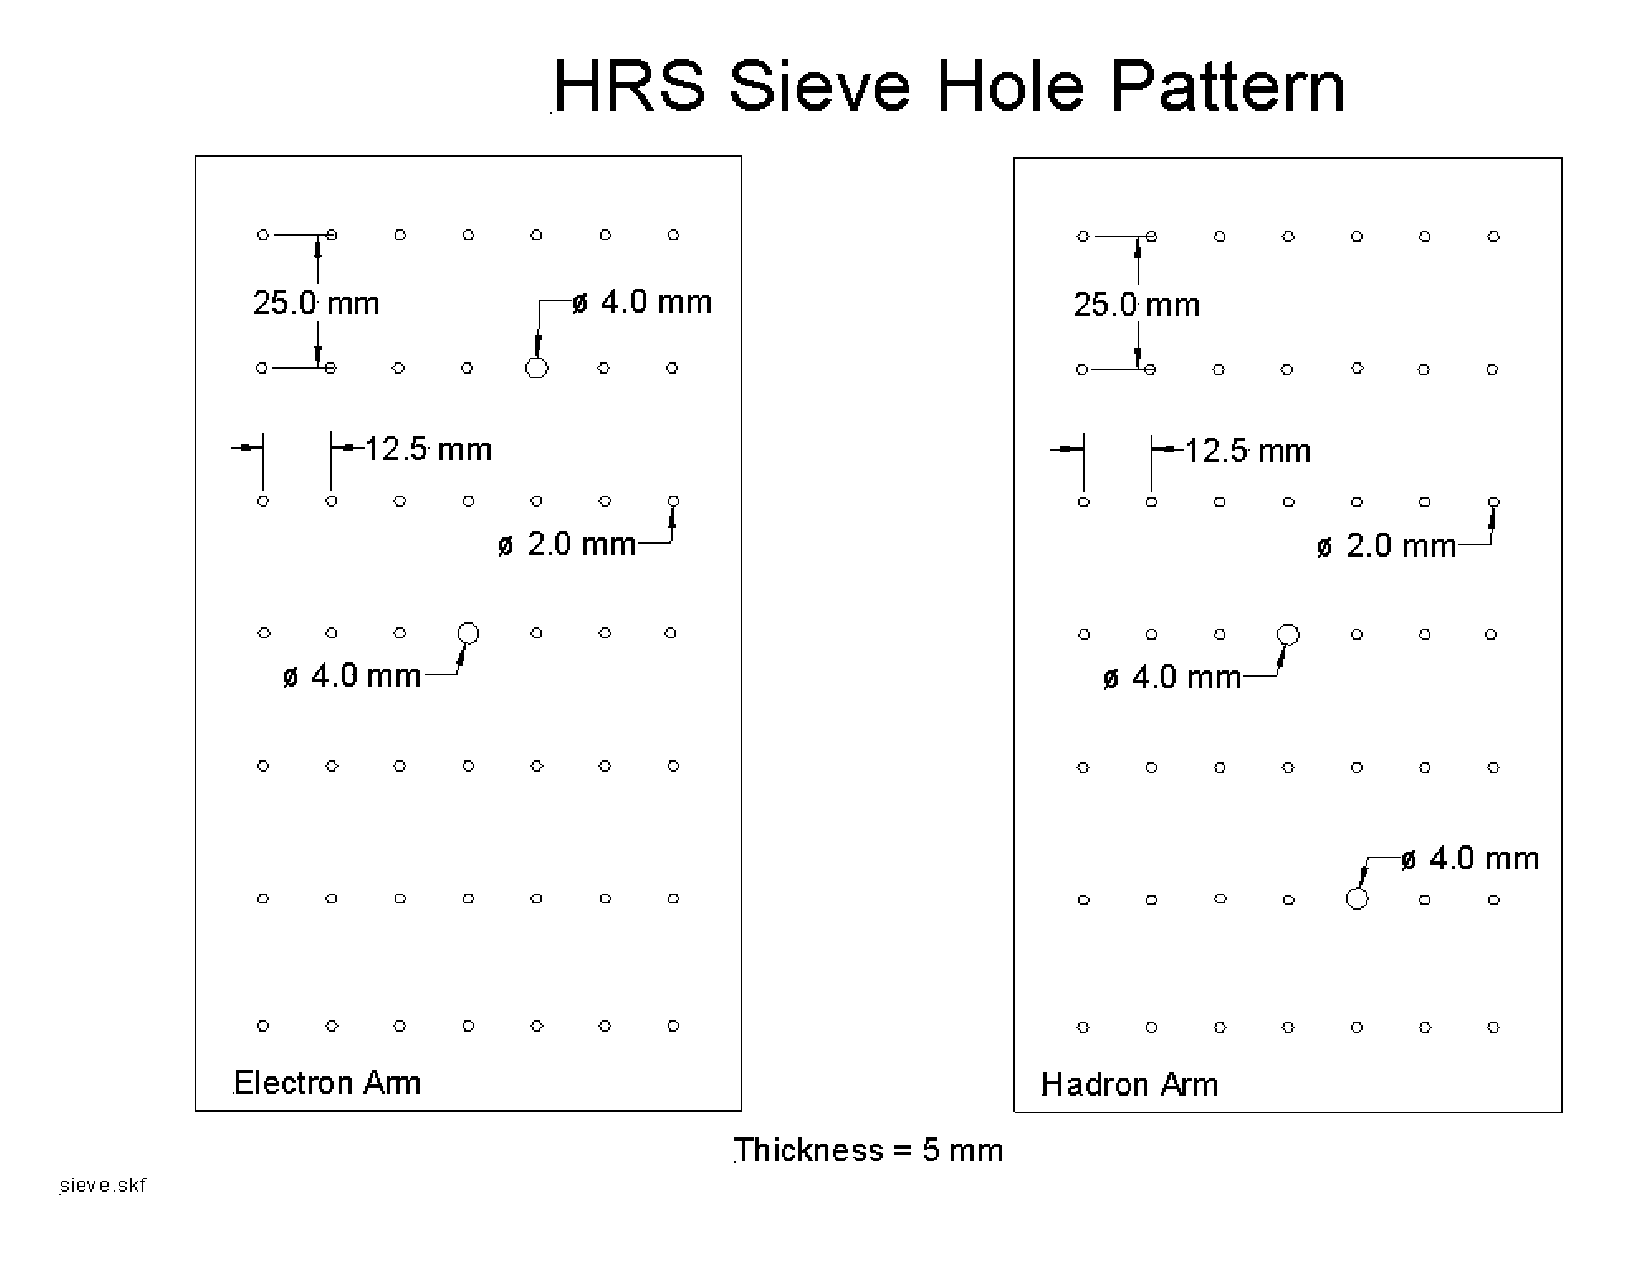
\includegraphics[type=pdf,ext=.pdf,read=.pdf,width=0.85\textwidth]{./figures/optics/sieve}
    \caption[Design of sieve slit plates]{\footnotesize{The design of sieve slit plates. Both arm have the identical plates but different mounting system. The graphic is taken from Hall A web-page.}}
    \label{sieve_slit}
  \end{center}
\end{figure}

As given in table~\ref{optics_data_table}, a set of optics data has been taken during the experiment with the optics target for $y_{tg}$ calibration. When taking angular calibration data, a sieve slit plate (Fig.~\ref{sieve_slit}) was installed at the entrance at Q1 for each HRS. The data was taken in the QE region to ensure each hole of the sieve slit plate had enough events. 
\begin{table}[!ht]
  \centering
  \begin{tabular}{|c||c|c|c|c|c|c|}
    \hline
    Run Number & Target   & Angle    & $P_{0} / P_{0}^{RQ3}$ (GeV/c)  & Raster & Sieve & Comment\\
    \hline \hline
    3695    & Dummy4cm & $23^{\circ}$ & 2.678/2.3492  &  Off   &  Out  & $\delta p$ +3\% \\
    \hline
    3698    & Dummy4cm & $23^{\circ}$ & 2.600/2.2808  &  Off   &  Out  & $\delta p$ 0\% \\
    \hline
    3704    & Dummy4cm & $23^{\circ}$ & 2.522/2.2124  &  Off   &  Out  & $\delta p$ -3\% \\
    \hline
    3700    & Multi-C  & $23^{\circ}$ & 2.600/2.2808  &  Off   &  Out  & \\
    \hline
    3701    & Multi-C  & $23^{\circ}$ & 2.600/2.2808  &  On    &  Out  & \\
    \hline
    4201-4205& Multi-C    & $25^{\circ}$ & 2.505/2.1975 & Off    &  In & \\
    \hline 
  \end{tabular}
  \caption[Run list of optics data.]{Run list of optics data, where Dummy4cm means two dummy foils separated by 4 cm, and Multi-C means the optics target with seven carbon foils. Two HRSs took data simultaneously with the same settings.}
  \label{optics_data_table}
\end{table}
\begin{figure}[!ht]
  \begin{center}
    \subfloat[Before optics calibration]{
      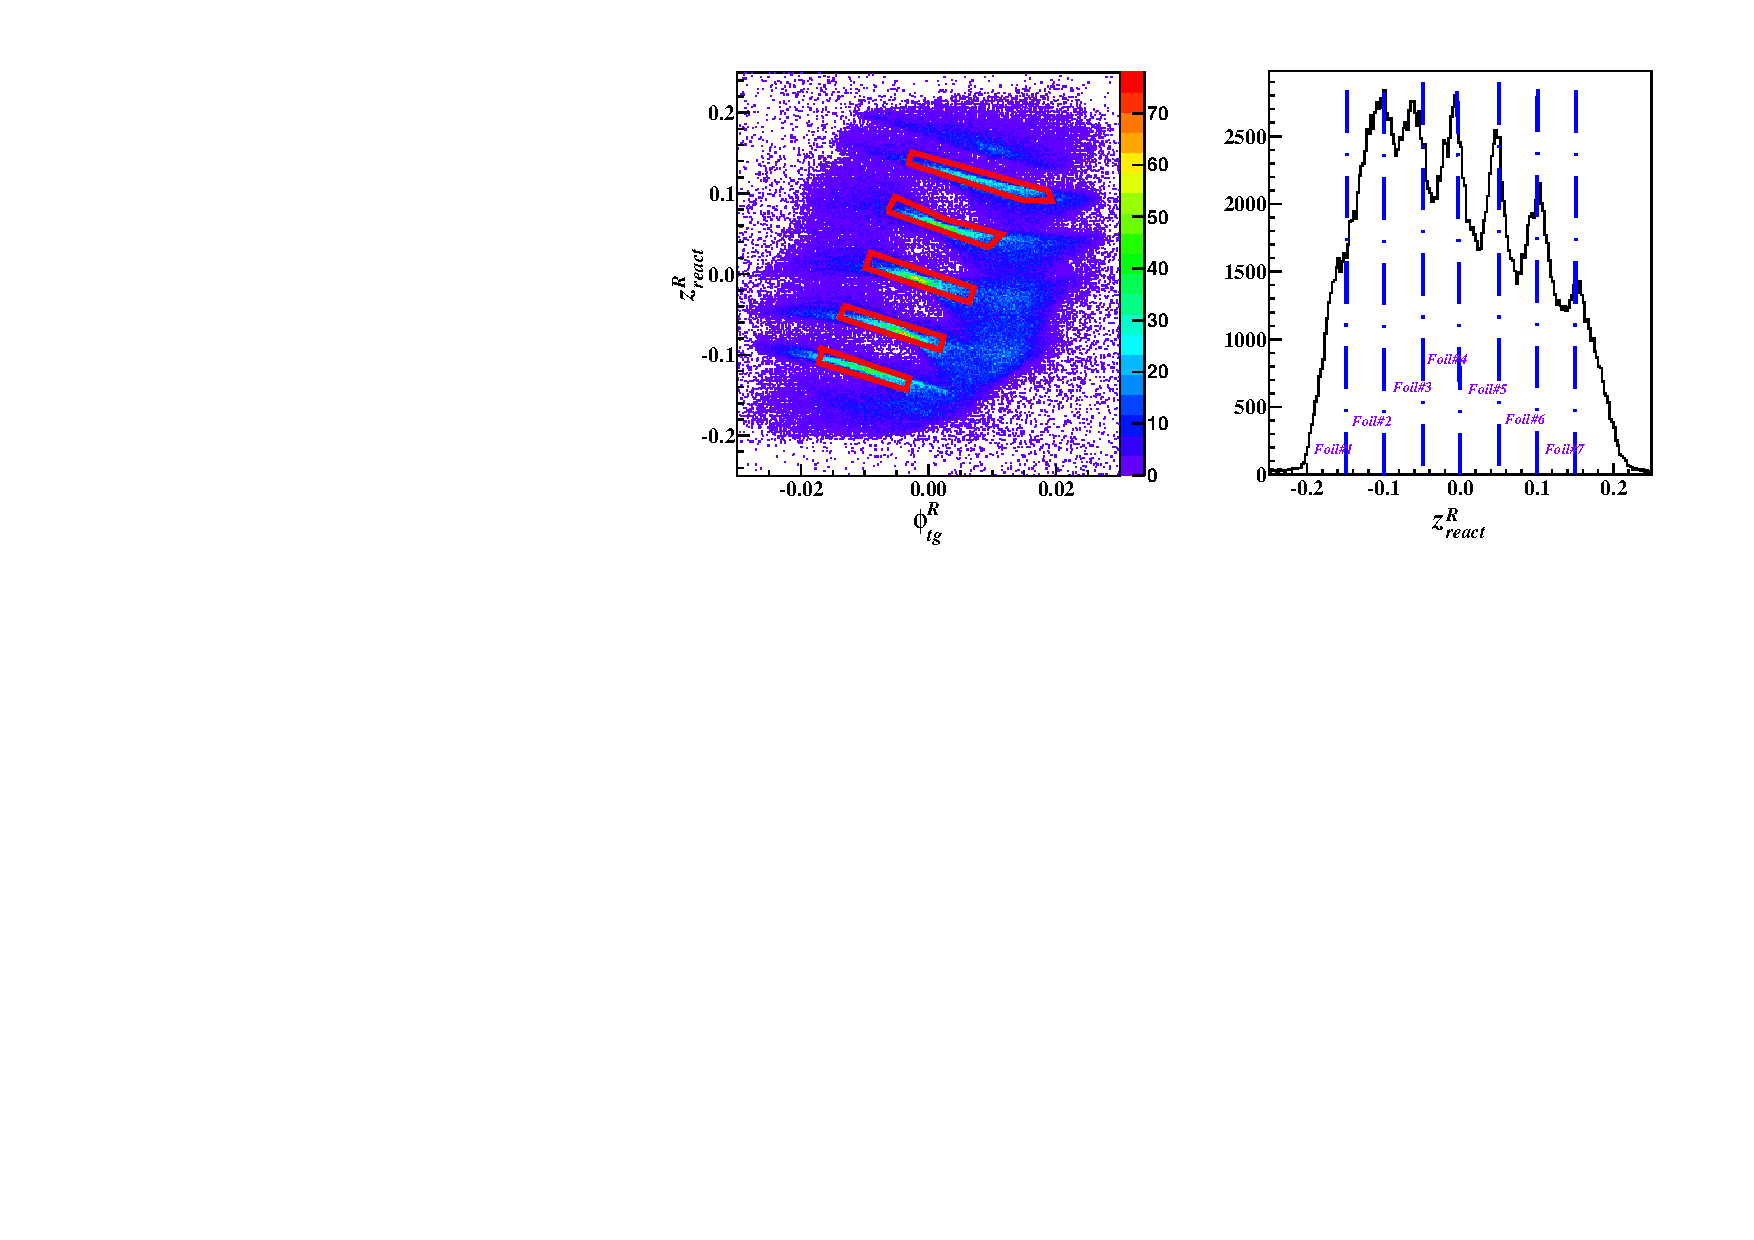
\includegraphics[type=pdf,ext=.pdf,read=.pdf,width=1.0\textwidth]{./figures/optics/R_VZ_Before}
      \label{vz_before}
    }
    \\ 
    \subfloat[After optics calibration]{
      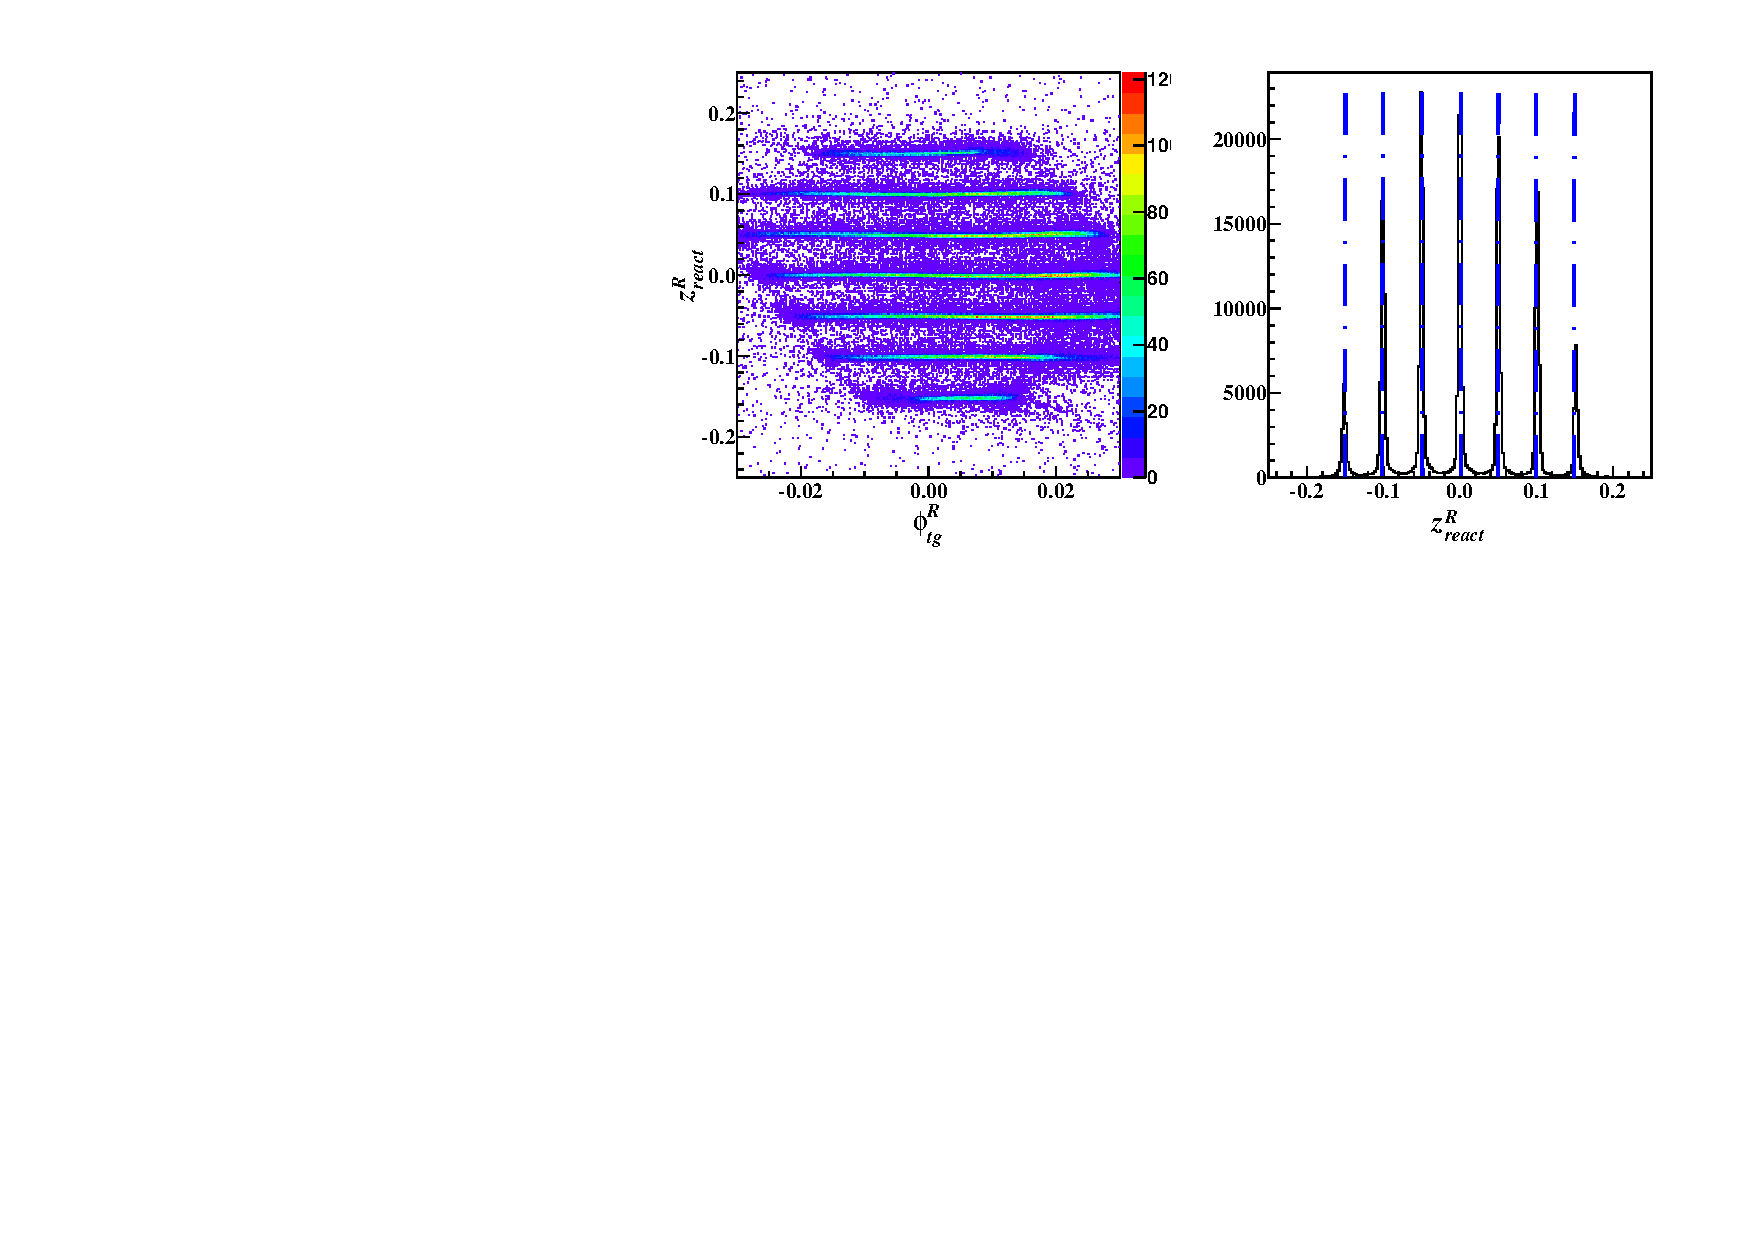
\includegraphics[type=pdf,ext=.pdf,read=.pdf,width=1.0\textwidth]{./figures/optics/R_VZ_After}
      \label{vz_after}
    }
    \caption[$Z_{react}$ distribution before and after the optics calibration]{\footnotesize{$Z_{react}$ distribution before and after the optics calibration. The 2-D plots reveal that each strip represents electrons scattered from the corresponding foil indicated in the 1-D plots. The red boxes in the first 2-D plot represent graphic cuts applied to selected good electron samples during the first iteration of the Y-terms calibration.}}
    \label{optics_vertex}
  \end{center}
\end{figure}

 The optics matrices used to replay optics calibration data were from previous experiments which shared similar spectrometer settings as this experiment. The initial HRS-L matrix taken from E05-102~\cite{jinge_thesis} was able to reconstruct the target plane quantities with good accuracy. The matrix was refitted by using the calibration data and the updated offsets from survey reports. The HRS-R optics matrix used by previous experiments, however, performed poor reconstruction of the target plane quantities because of the mis-tuned RQ3 field, as shown in Fig.~\ref{vz_before} and Fig.~\ref{sieve_before}. The detailed procedure to calibrate the new HRS-R optics matrix will be discussed. 

 Due to the change of the RQ3 field, the higher order effect of the HRS-R optics may be different from the one with normal RQ3 field and could change the number of elements and their values in the matrix. In addition to the old matrix elements, new matrix elements were added in the optics terms to form a complete set of polynomials up to the 5th-order, but their values were initially set to zero. After the calibration data was replayed with this optics matrix, events selection at the focal plane was performed to select event from main trigger (T1). The one-track cut on VDCs and PID cuts on the GC and calorimeters were applied to select electrons only. Events at the edge of HRS acceptance were eliminated by choosing only the flat regions of the focal plane quantities. 

Events from Run-3700 were used to calibrate the matrix elements in Y-terms (Eq.~\eqref{optics_eq}). When one plots the 2-D histogram of $z_{react}$ versus $\phi_{tg}$ (Fig.~\ref{vz_before}), events scattered from a specific foil form a strip where both ends  were smeared due to the defocusing effect from RQ3. The first iteration was to select electron samples which clearly belong to a certain strip (e.g. near the center of each strip as included in the red boxes in Fig.~\ref{vz_before}), while events in the overlap regions were discarded. For each sample, its $z_{react}$ value was assigned with the position of the foil it belonged to. After the offsets in Table~\ref{optics_offset_table} and Table~\ref{sieve_offset_table} were applied in the calibration, the matrix elements in Y-terms were fitted by an optimizer based on the Minuit minimization method~\cite{jin_huang_optics}. The high order elements in Y-terms were removed one by one until the minimization started to fluctuate. The data was replayed with these new matrix elements and the big improvement of $z_{react}$ distribution is demonstrated in Fig.~\ref{vz_after}.
\begin{figure}[!ht]
  \begin{center}
    \subfloat[Before optics calibration]{
      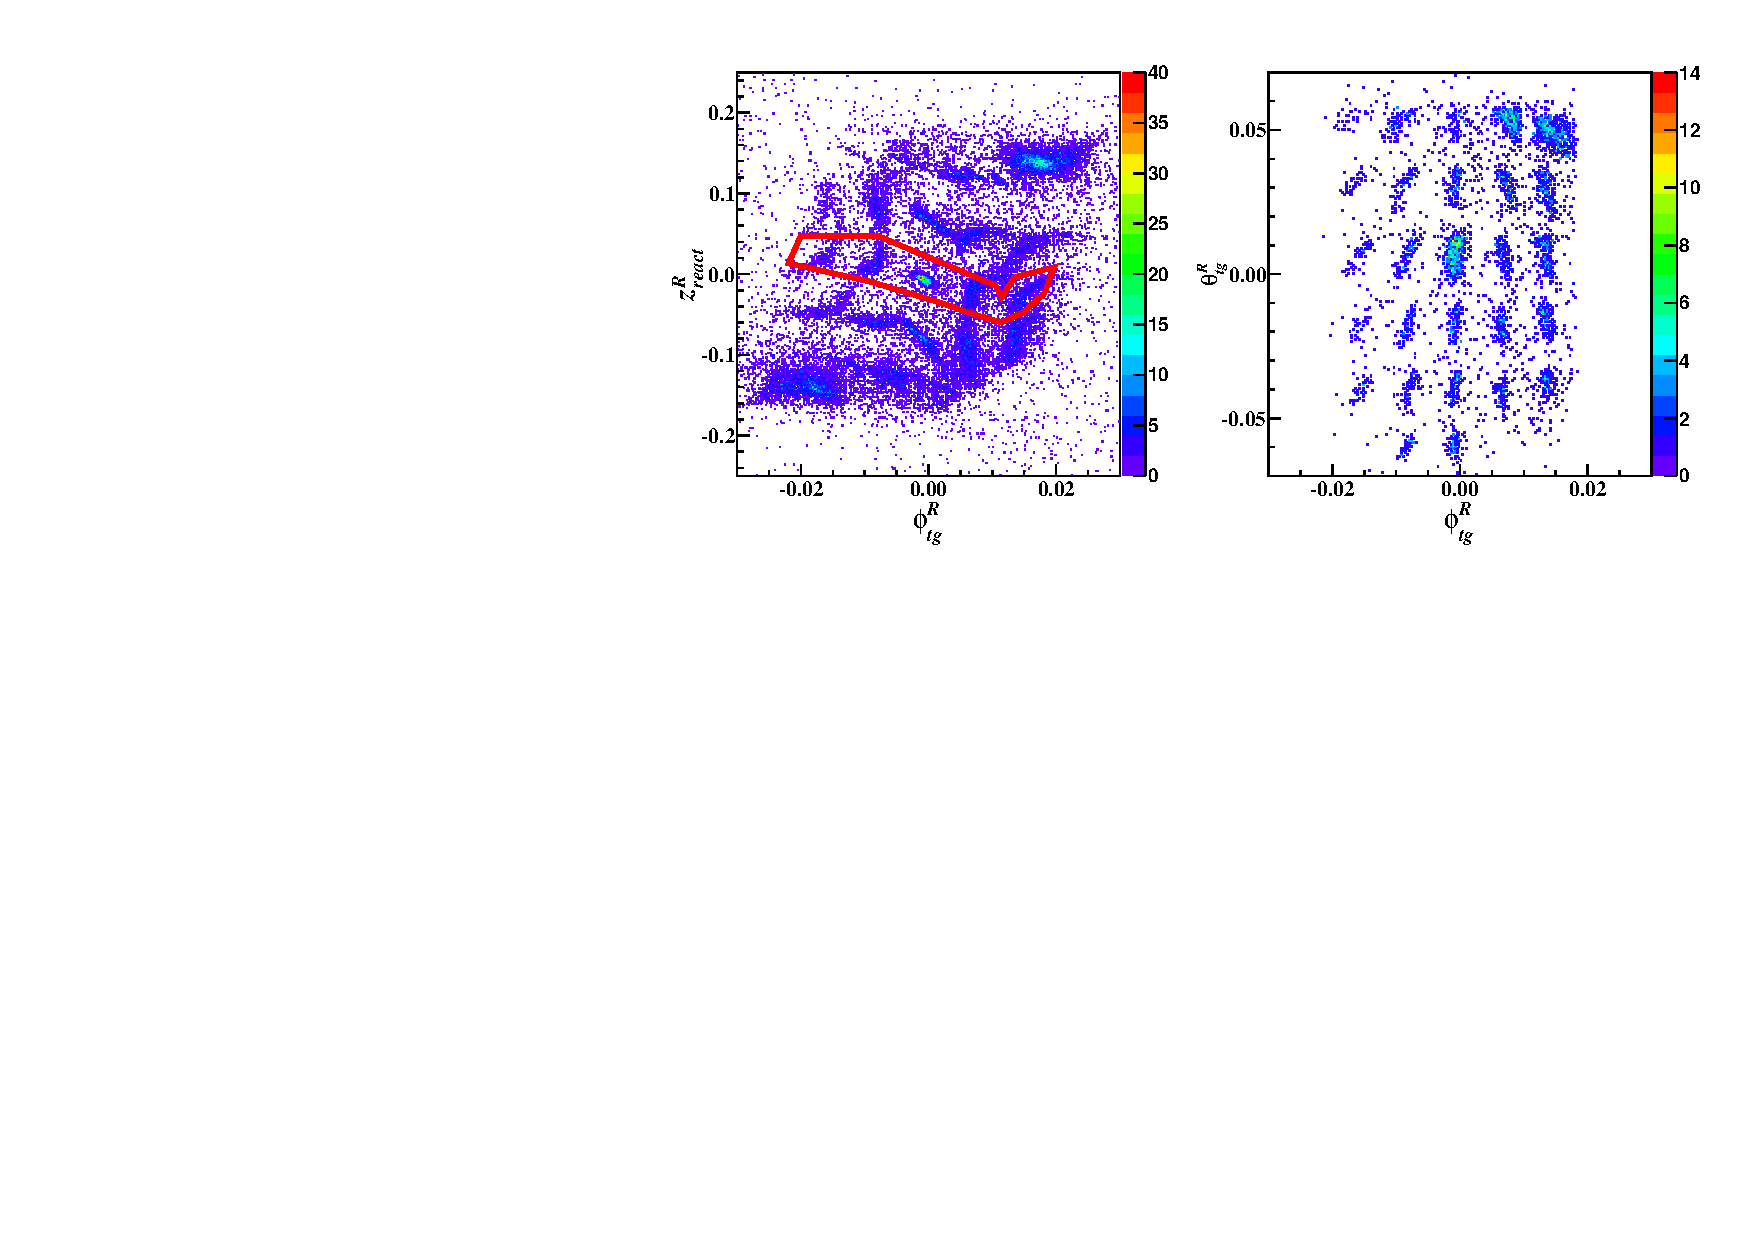
\includegraphics[type=pdf,ext=.pdf,read=.pdf,width=1.0\textwidth]{./figures/optics/R_SS_Before}
      \label{sieve_before}
    } 
    \\
    \subfloat[After optics calibration]{
      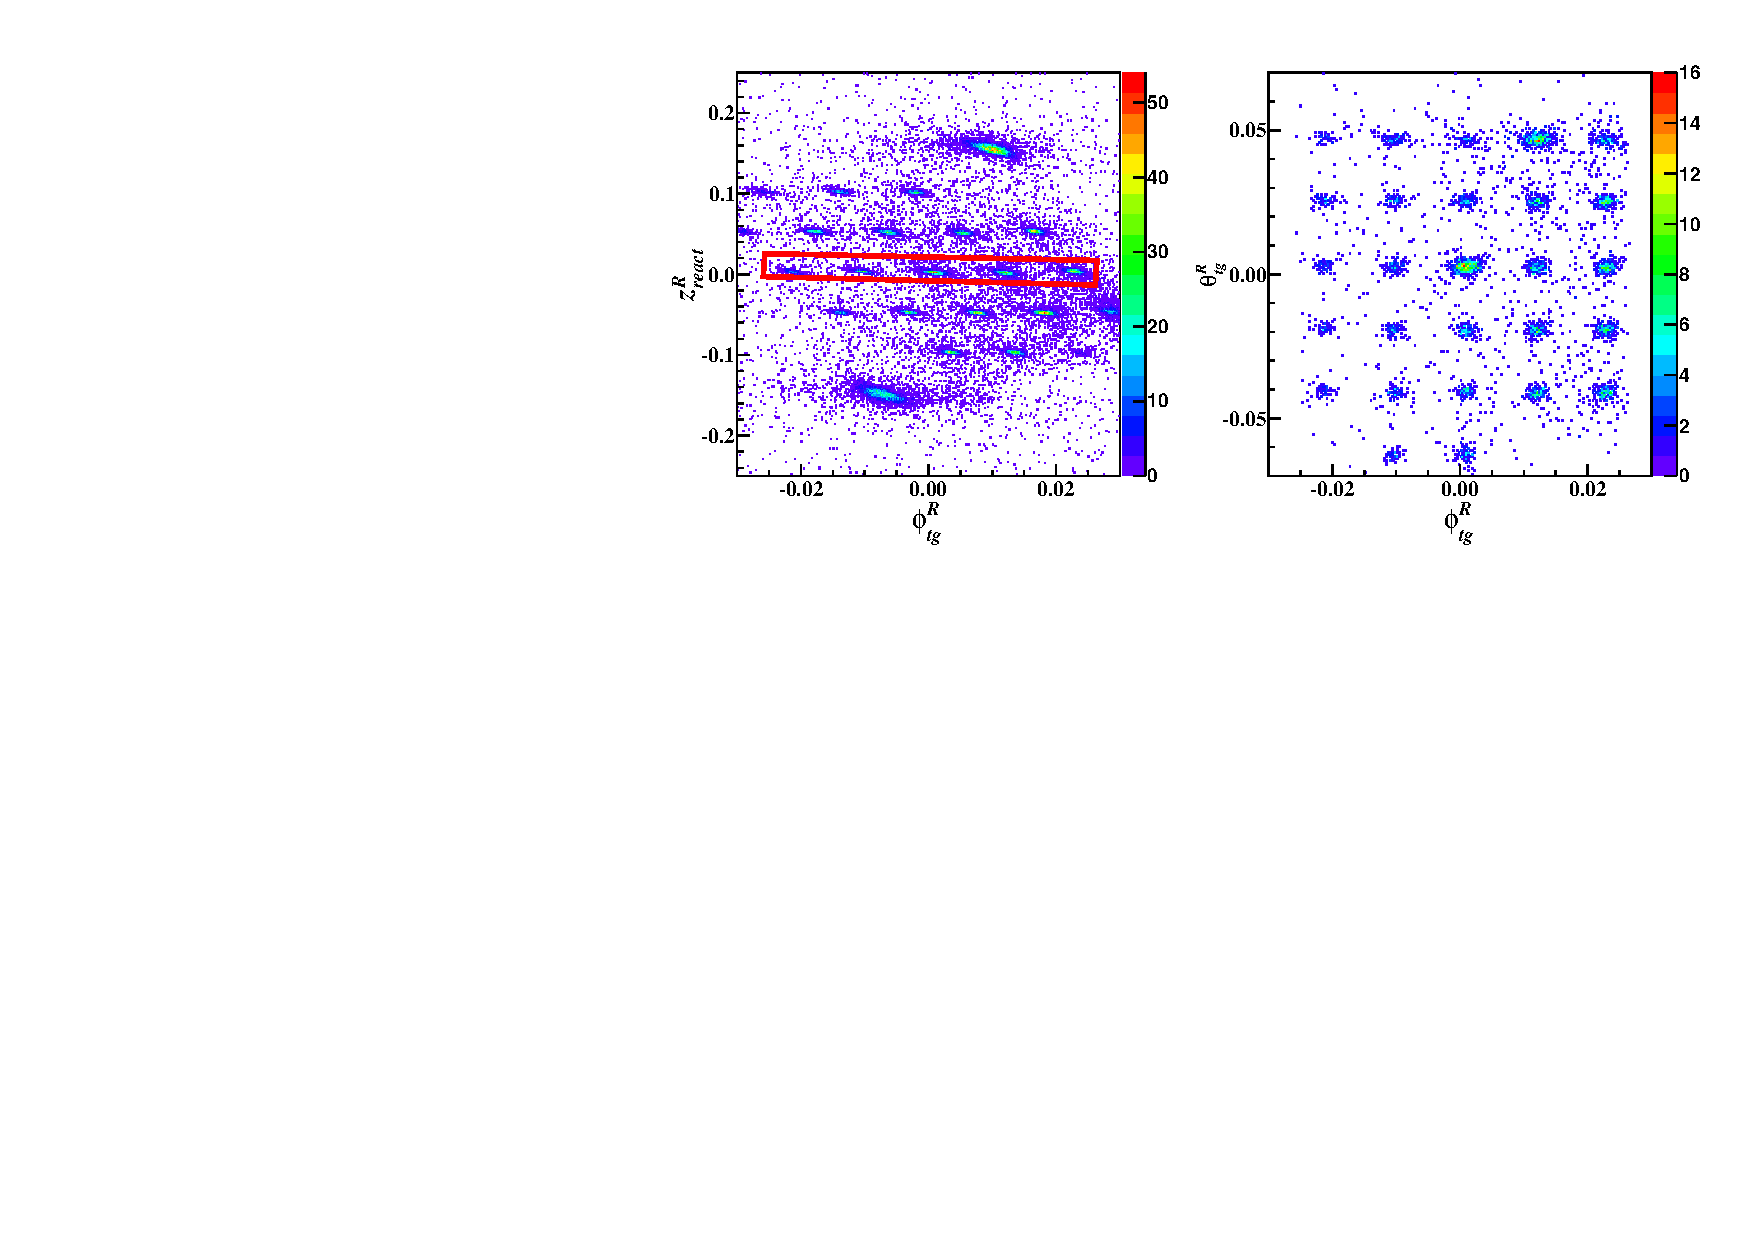
\includegraphics[type=pdf,ext=.pdf,read=.pdf,width=1.0\textwidth]{./figures/optics/R_SS_After}
      \label{sieve_after}
    }
    \caption[Sieve slit pattern before and after the optics calibration]{\footnotesize{$Z_{react}$ Sieve slit pattern before and after the optics calibration. Cutting on a single foil (the red box) is required to see the clear sieve slit pattern. Events from each hole are individually extracted and assigned with the values of $\theta_{tg}$ and $\phi_{tg}$ at the center of the hole.} }
    \label{optics_sieve}
  \end{center}
\end{figure}

The procedure of calibrating T-terms and P-terms was similar but used calibration data taken with a sieve slit plate (Runs 4201-4205). Since Y-terms have been optimized, these sieve slit runs were first replayed with new elements of Y-terms updated in the DB. The sieve slit patterns shown in a 2-D plot of target plane quantities $\theta_{tg}$ and $\phi_{tg}$ were compared with the design of the sieve slit plate in Fig.~\ref{sieve_slit}. On the right plots of Fig.~\ref{optics_sieve}, each spot corresponds to the one sieve slit hole. For an electron sample that could be clearly identified from a spot, the coordinate of this event on the sieve slit plane, ($x_{ss}$, $y_{ss}$), was set at the center of the hole since the diameter of the hole is very small (2 mm). The values of $\theta_{tg}$ and $\phi_{tg}$ can be directly calculated from the values $x_{ss}$ and $y_{ss}$.

 The matrix elements of T-terms and P-terms were fitted separately with the same optimizer and unnecessary matrix elements were removed by checking the variation of the minimization Chi-Square. Fig.~\ref{sieve_after} shows that the sieve slit holes were well aligned after the calibration of angular terms. 

 With updated Y-terms, T-terms and P-terms in the data base, the calibration runs were replayed again. As the target plane quantities were reconstructed with higher resolutions and the events were better separated, the second iteration was processed with more good samples. The calibration was completed when the minimization Chi-Square started to fluctuate after several iterations. 

 The calibration of D-terms requires data to be taken with the central momentum intentionally shifted by small values, for example, by $\mathrm{\pm 3\%}$. However, the experiment was running in the QE region and the peak of the momentum distribution was too broad and insensitive to these small offsets. Without the elastic data, the D-terms could not be calibrated. In Appendix C, a different method was discussed to obtain the correct $\delta p$ reconstruction.